% Overizcht feest:
% Datum \$DATUMFEEST
% Aantal gasten \$GROEPGROTE
% Waarvan kinderen \$KINDEREN
% Betreft: \$BETREFT
% Begintijd: \$BEGINTIJD
% \$STARTPLANNING

\documentclass{scrartcl}
\usepackage[dutch]{babel}
\usepackage{fancyhdr}
\usepackage{wallpaper}
\usepackage[official]{eurosym}

\graphicspath{{img/}}
\def\infofoot{
	\fancyfoot[C]{
		\large Restaurant De Huiskamer \\
	\tiny Kerkdijk 2 - $7964KB$ Ansen - tel 0522-471280 - KvK 04005343
	 -  info@dehuiskamer.com \\
	IBAN NL07 SNSB 095.65.49.721 - BTW nr: 8094.43867B01
	\\
www.dehuiskamer.com - www.de2dekamer.nl - m.facebook.com/RestaurantDeHuiskamer
}
\fancyfoot[R]{
    \parbox[b]{0cm}{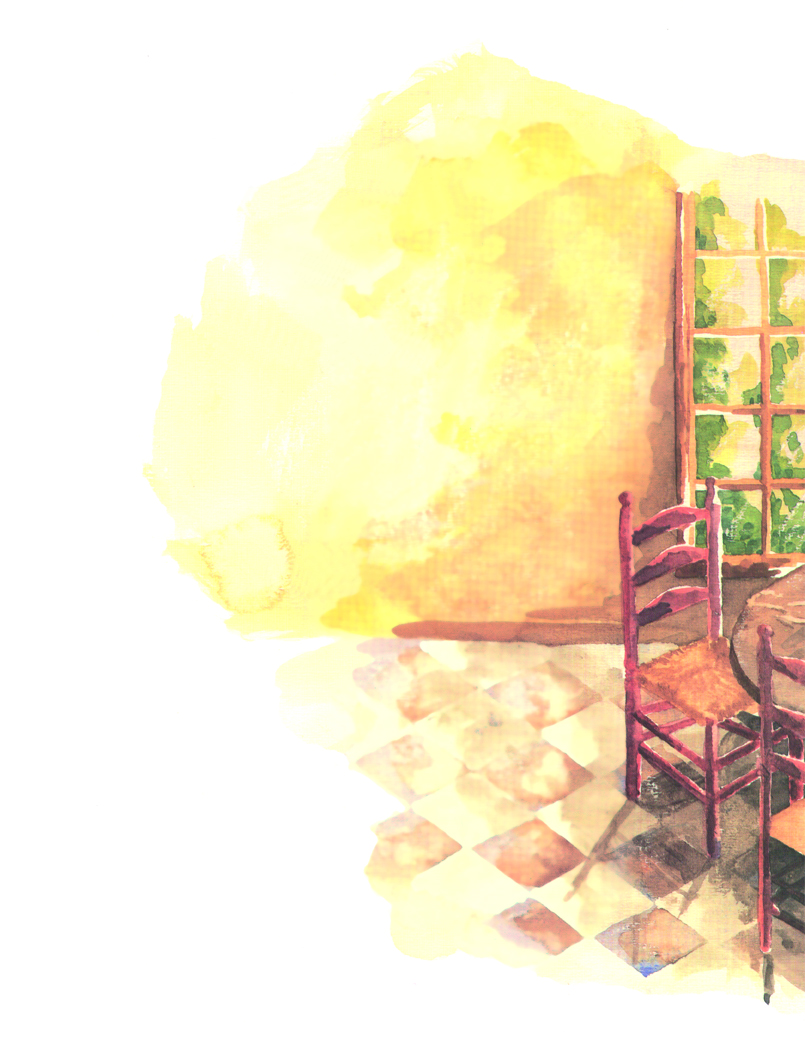
\includegraphics[scale=0.12]{logo2kleur}}%
}
}
\fancypagestyle{footer}{%
	\fancyhf{}
	\infofoot
}
\pagestyle{fancy}
\renewcommand\headrulewidth{0pt}
\chead{\large Restaurant De Huiskamer \\
\small Ansen $\quad$ tel $0522-471280$}
\infofoot
\begin{document}
\ThisURCornerWallPaper{0.25}{img/logo.jpg}

\title{Restaurant De Huiskamer}
\date{Ansen, \today}
\maketitle
\thispagestyle{footer}

\begin{flushright}
	\$NAAM \\
	\$ADRESS \\
	\$POSTCODE \$PLAATS
\end{flushright}
\section*{Betreft: offerte}
\begin{tabular}{l r}
  E-mail & \$EMAIL  \\
  Tel & \$TEL  \\
\end{tabular}

\subsubsection*{Geachte \$NAAM,}

Naar aanleiding van ons gesprek ontvangt u hierbij een vrijblijvende offerte
voor \$BETREFT op \$DATUMFEEST

Uitgaande van \$GROEPGROTE gasten \$KINDEREN kan dit er als volgt uit zien:

\$DRAAIBOEK

\newpage

\$PRIJSOVERZICHT

\end{document}
